\chapter[How Selection Changes a Population]{How Selection Changes a Population --- The Outward Results}
\label{cha:how-selection-changes-population-outward-results}

Although the genes are the units of inheritance, the animal is the
smallest unit which can be selected or rejected at any one time. Selection
may be between still larger units such as families, inbred lines,
breeds, races, etc., but that is optional. The breeder may study the different
characteristics of each animal as separately as he will, and may
like some of its characteristics very much and dislike others of its characteristics
at the same time, but what he does with the animal applies to
all its characteristics, the admired ones as well as the disliked ones.

The animal is selected or rejected for breeding according to the
breeder's opinion of how much its meritorious characteristics outweigh
its weaknesses, and in comparison with the other animals which are
available £or him to use in case this one were rejected. It is thus convenient,
when considering the general consequences of selection as the
breeder sees them, to consider selection as being made for net merit as if
that were a single characteristic. Of course net merit is a compound
characteristic affected by many genes, but so too are most measurable
characteristics, such as weight, wither height, egg production, litter
size, etc. Net merit is also likely to change in definition as economic
conditions change, or when one characteristic in the breed improves so
much that variations in it become less important than they once were.
Also breeders will not entirely agree on the ideal toward which they are
striving and on the actual importance of different variations. The yard sticks
for measuring net merit are thus somewhat elastic, changing a bit
from time to time and from place to place and according to the varied
purposes for which the animal s are to be used. These are important
practical difficulties in measuring net merit £or each animal in an objective
way so that all would agree on the merit of each animal. Yet the
general idea of net merit is as easily understood as the idea of obtaining
an individual's net income by subtracting his losses in some enterprises
from his gains in the others, or obtaining an individual 's net worth in a
financial statement by adding his various assets and subtracting his liabilities
from them.

Figure~\ref{fig:Lush_Figure_17} shows two diagrams of the way selection might
take place. The kind of selection pictured in \textit{A} corresponds to that actually
practiced for important traits in stock breeding where many different
traits must be considered. Some animals which are mediocre or even
inferior in the characteristic pictured are saved because they are unusually
desirable in several other characteristics or because the breeder is
careless or confused. That pictured in \textit{B} is the extreme kind of selection
which might be practiced in a laboratory experiment on selection for
one trait alone, disregarding all others. The selection practiced in livestock
breeding can be like that pictured in B, if the net merit of the animal
as a whole is the characteristic which is measured along the horizontal
axis in \textit{B}. The kind of selection pictured in \textit{B} is, of course, more
effective if the percentage saved is the same as in \textit{A}.

\begin{figure}
	\centering
    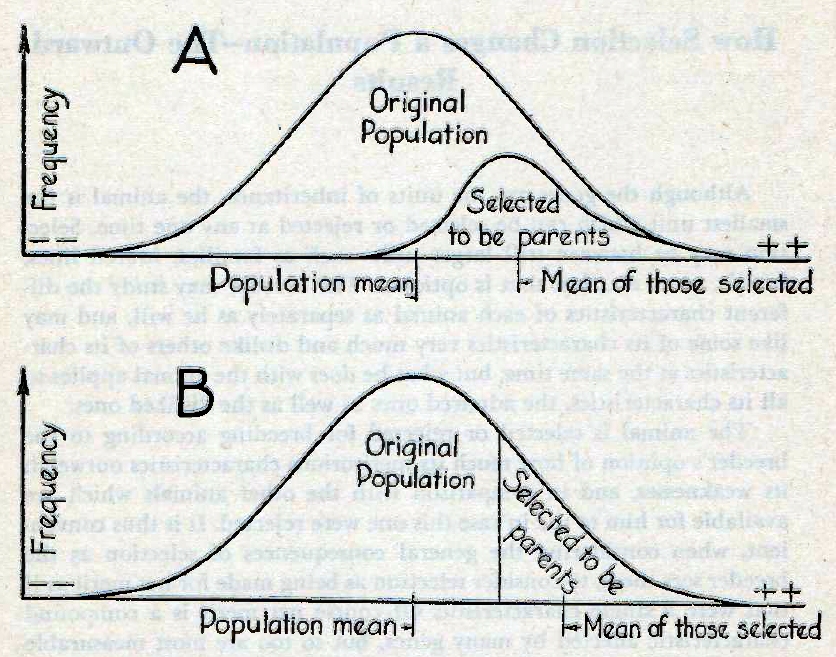
\includegraphics[width=\textwidth]{Figure_17.png}
    \caption{Two ways in which the merits of those chosen to be parents by rather
			 intense selection might be distributed with respect to the merit of the original population
			 from which they were taken. The better individuals are to the right, the poorer
			 to the left. A indicates the usual kind of selection where at least a few mistakes are
			 made and where some attention must be paid to characteristics other than the one
			 for which merit is indicated here. B is the most extreme form of selection conceivable.
			 No mistakes are made and selection is entirely for the characteristic for which
			 degrees of merit are indicated along the horizontal scale.}
    \label{fig:Lush_Figure_17}
    \index{Generation interval}
\end{figure}

\section*{THE SELECTION DIFFERENTIAL}
\index{Replacement rates|(}
\index{Selection!differential|(}

The most useful measure of the intensity of the selection actually
practiced is the difference between the average of those selected to be
parents and the average of the whole population in which they were
born. It is convenient to speak of this superiority of the selected parents
as the ``selection differential.'' As a numerical example, if a herd of gilts
in their first litters farrow an average of 8.6 pigs and we select for large
litter size intensely enough that those which are kept for further breeding
averaged 9.5 pigs in the first litters, then the selection differential
for litter size at this particular \index{Culling levels|(}culling was 9.5 minus 8.6 or .9 pig. The
selection differential which can be attained is sharply limited by the fact
that enough offspring must be saved to replace the parents in any breed
stationary in numbers. More than that must be saved in a breed which
is increasing in numbers. Reproductive rates and percentages of deaths
and other losses from controllable and uncontrollable causes differ
among species of farm animals. Table~\ref{tbl:Lush_Table_11} shows what are believed
to be reasonable figures for the usual percentage of offspring which must be
saved for replacement purposes. The vital statistics of farm animals are
not well enough known to make these estimates as accurate as they
should be. Of course, there is some variation in the replacement rates
from year to year and from farm to farm as conditions of health and
management vary.

Table~\ref{tbl:Lush_Table_12} shows for selection such as that pictured in
\textit{B} of Figure~\ref{fig:Lush_Figure_17} how much the parents can
average above the whole population from which they were selected.\footnote{Table~\ref{tbl:Lush_Table_12}
is for a \textit{normally distributed} population. Most animal breeding
populations are nearly enough normal that these figures are sufficiently accurate to be
useful. Where a few arc culled from the long ``tail'' of a distinctly skew curve, the
gain will be more than is indicated in the upper lines of Table~\ref{tbl:Lush_Table_12},
but gains from the heavier culling shown in the bottom line<1 will he less.}
It thus gives \textit{the maximum} selection differential which could be attained in a
whole breed if the percentage of the population which must be saved for replacement
were the only limiting factor. The selection differential in Table~\ref{tbl:Lush_Table_12}
is expressed in terms of standard deviations, so as to be applicable to all kinds of
characteristics.

\begin{table}[htbp]
	\centering
	\caption{\textsc{Estimated Replacement Rates Which Limit Breed\\Improvement}}
	\label{tbl:Lush_Table_11}
	\begin{tabular}{L{2.5cm}|C{3.5cm}|C{2cm}|C{2cm}}
		\hline
		\hline
%		\multirow{5}={Kind of Animal} & \multirow{5}{2.5cm}{Average Interval Between Generations (i.e., Average Age of Parents When Their Offspring Are Born)} & \multicolumn{2}{C{6cm}}{\multirow{4}={Percentage of Progeny Reared Which Are Needed for Replacements in a Population Static Numbers}} \\
		& Average Interval &
		\multicolumn{2}{C{5cm}}{ } \\
		& Between &
		\multicolumn{2}{C{5cm}}{ } \\
		& Generations &
		\multicolumn{2}{C{5cm}}{Percentage of Progeny} \\
		& (i.e., Average & 
		\multicolumn{2}{C{5cm}}{Reared Which Are} \\
		& Age of Parents &
		\multicolumn{2}{C{5cm}}{Needed for Replacements} \\
		& When Their &
		\multicolumn{2}{C{5cm}}{in a Population} \\
		& Offspringx &
		\multicolumn{2}{C{5cm}}{Static in Numbers} \\
		\cline{3-4}
		Kind of Animal	& Are Born)	& Females	&	Males \\
		\hline
		Horses			& 9 to 13 years					& 35 to 45	& 2 to 4	\\
		Beef cattle		& 4\nicefrac{1}{2} to 5 years	& 40 to 50	& 3 to 5	\\
		Dairy cattle	& 4 to 4\nicefrac{1}{2} years	& 50 to 65	& 4 to 6	\\
		Sheep			& 4 to 4\nicefrac{1}{2} years	& 45 to 55	& 2 to 4	\\
		Swine			& About 2\nicefrac{1}{2} years	& 10 to 15	& 1 to 2	\\
		Chickens		& About 1\nicefrac{1}{2} years	& 10 to 15	& \nicefrac{1}{2} to 2	\\
		\hline
	\end{tabular}
\end{table}

An example will show how Tables~\ref{tbl:Lush_Table_11} and \ref{tbl:Lush_Table_12} are used. The standard
deviation of the weights of fleeces shorn in the same year from a group
of Rambouillet sheep described in Technical Bulletin 85 of the United
States Department of Agriculture is about l.86 lbs. (See Table 2 in that
bulletin.) If a hitherto unculled group of such ewes and rams were to be
culled solely on fleece weight at a single shearing, the 50 per cent of the
ewes which it would be necessary to save would excel the flock average
by .80 times the standard deviation, or 1.49 pounds of wool. The 3 per
cent of the rams with the heaviest fleeces would excel the average for
all rams by 2.27 times the standard deviation, or 4.22 pounds of wool.
Since inheritance is practically equal from sire and dam, this would
make a selection differential of 2.86 pounds of wool at that one shearing,
so far as the next generation is concerned.
\noclub[3]
\index{Replacement rates|)}

\section*{INCREASE TO BE EXPECTED IN THE POPULATION MEAN}
\index{Environment and heredity|(}

The next generation would be expected to be about as variable as
the preceding one, but to average outwardly whatever their parents
averaged genetically. In case the genes all combined their effects additively
and the existing environmental variations did not affect the characteristic
at all, the genetic average of the parents would be the same as
their phenotypic average, the offspring would average whatever their
selected parents did, and the increase in the population mean per generation
would be equal to the selection differential (see Figure~\ref{fig:Lush_Figure_18}).
Actually the permanent improvement in the population average each
generation will be only a fraction of the selection differential.
\index{Additive effects of genes} That fraction
has for its numerator the additively genetic variance (Chapter 7)
and for its denominator the actual variance\index{Variance}; i.e., the fraction is
$\frac{\sigma_G^2}{\sigma_G^2 + \sigma_D^2 + \sigma_I^2 + \sigma_E^2}$ which for
brevity we may call the \index{Heritability|(}``heritability'' of the differences which existed in the
parental generation before selection began. In addition, \index{Epistatic effects|(}
epistatic differences
will cause temporary gains which in amount are less than half of
$\frac{\sigma_I^2}{\sigma_G^2 + \sigma_D^2 + \sigma_I^2 + \sigma_E^2}$ of the
selection differential. These gains from selecting for epistatic differences
tend to disappear in future generations as the genes recombine. They
can be maintained only by continued selection.

\begin{table}
	\centering
	\caption{\textsc{Selection Differential (in Terms of Standard Deviations) Attainable by Various Intensities of Selection}}
	\label{tbl:Lush_Table_12}
	\begin{tabular}{C{5cm}|C{5cm}}
		\hline
		\hline
		Percentage of Population Saved	& Selection Differential 	\\
		\hline
		.90								& .20						\\
		.80								& .35						\\
		.70								& .50						\\
		.60								& .64						\\
		.50								& .80						\\
		.40								& .97						\\
		.30								& 1.16						\\
		.20								& 1.40						\\
		.10								& 1.75						\\
		.05								& 2.06						\\
		.04								& 2.15						\\
		.03								& 2.27						\\
		.02								& 2.42						\\
		.01								& 2.67						\\
		\hline
	\end{tabular}
\end{table}

In the example of selection concentrated on fleece weight, the
increase in average fleece weight per generation would be 2.86 pounds
per generation in the impossibly extreme case in which all differences in
the parental generation were additively genetic, 1.43 pounds per generation
in case heritability of differences is 50 per cent, and only .95
pounds per generation in the more probable case that heritability of
differences in shearing weights is about one-third. The annual increa se
in the flock average would be about one -fourth or fifth of these increases
\textit{per generation}, since the interval between generations, the average age
of the parents when the lambs are born, is about four or five years.
\index{Selection!differential|)}

This example is somewhat artificial for farm animals in that it
assumes that all selection would be practiced at one stage in each generation.
Actually, only a few of the rams born would be kept as rams
even until the first shearing. Many of the ewes would be culled after the
second shearing, others would be culled after the third shearing, others
after the fourth, etc., some culling taking place all through the lifetime
of that band of sheep and much of the culling being based on things
other than fleece weight. All these things operate to lessen the intensity
of the culling which could be done at any one time and to render difficult
the measurement of the intensity of the selection actually practiced.
The example illustrates the general principles that the intensity
of selection possible is sharply limited by the necessity for replacements
and that the intensity of selection actually practiced is to be measured
in terms of the difference between the average of those saved for parents
and the average of the generation in which they were born. The
method of computing the selection differential in this example is fairly
well suited in actual practice to the case of an animal, or some of the
annual plants, where the generations do not overlap and where nearly
all the selection is practiced at one stage in the life cycle.
\index{Culling levels|)}
\nowidow

\section*{CONSEQUENCES OF INCOMPLETE HERITABILITY}

Some individuals are mistakenly saved or rejected for parents
because the effects of environmental variations make them appear
phenotypically better or worse than their genetic values. These environmental
effects are not transmitted to their offspring. Selection of the
phenotypically superior tends automatically to keep among those
saved more than a fair share of lhose which appeared phenotypically
better and less than a fair share of those which appeared phenotypically
worse than they were genetically. The environmental effects are left
behind when they reproduce. Their genes segregate from these combinations
to recombine in the unselected offspring to give a nearly fair
picture of the genetic worth of the parents.

Similarly where the favorable genes tend to be dominant the heterozygotes
will have been made to appear phenotypically better and the
homozygotes relatively worse than corresponds to their average breeding
value. The \index{Dominance}dominance deviations of a parent are not transmitted as
such to its offspring, since they are caused by the interaction of a pair
of allelic genes and only one gene out of each allelic pair can be transmitted
in any one gamete.

Epistatic effects, being dependent on combinations of nonallelic
genes, are transmitted to a portion of the offspring, that portion being
progressively smaller the more complex the combination. If \textit{A} and \textit{B}
are not linked but together have an effect which neither of them has
separately, that effect would be transmitted in about one-fourth of the
gametes from an \textit{AaBb} individual, whereas the additive effects of \textit{A}
would be transmitted in about half of the gametes. An epistatic effect
requiring the joint presence of three nonlinked genes, \textit{A}, \textit{B}, and \textit{C},
would be transmitted in only about one-eighth of the gametes from an
AaBbCc individual, etc. Even when such epistatic effects are transmitted,
the gene combinations responsible for them tend to segregate in
later generations, this process tending to continue until the genes are
combined at random. Hence the partial but transitory gains from selecting
for epistatic differences.

Figure~\ref{fig:Lush_Figure_18} shows what would be expected to happen in an experiment
on selecting for a perfectly hereditary character, with the selection
intensity such that in the high line only the upper half in each generation
were saved for parents, while in the low line only the lower half in
each generation were saved for parents. Obviously, even with such an
impossibly extreme case as perfect heritability (no effects at all by
environment, dominance, or epistasis), it will require several generations of
selection before all overlapping between the two lines ceases. Among
the offspring of selected parents there will always be some poorer than
the poorest of the parents although, if heritability were perfect, the
average of the offspring would equal the average of their selected
parents. The selected parents will not be much more or less homozygous
than the average of the population from which they came. They will
produce some gametes worse than are typical of them as well as some
which are better. When two inferior gametes unite, the result is an offspring
poorer than the poorest of those individuals which were saved to
be parents.

\begin{figure}
	\centering
    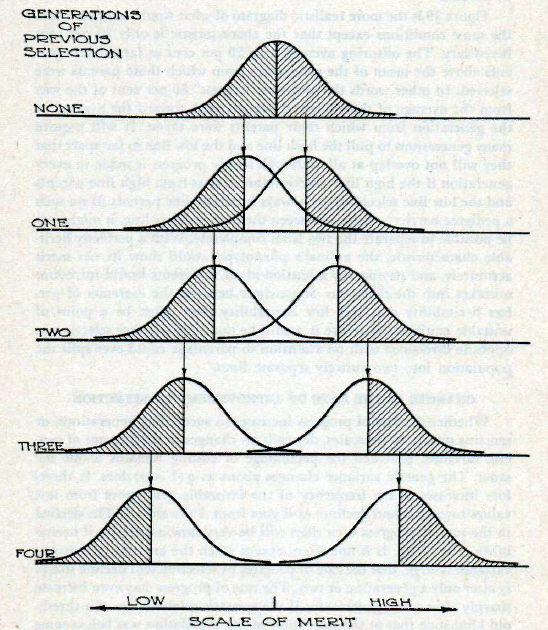
\includegraphics[width=\textwidth]{Figure_18.png}
    \caption{The results expected when selecting simultaneously a high and a low
			 line for a perfectly hereditary characteristic. In the high line the high half and in
			 the low line the low half in each generat1on are saved as parents.}
    \label{fig:Lush_Figure_18}
\end{figure}

Figure~\ref{fig:Lush_Figure_19} is the more realistic diagram of what would happen under
the same conditions except that the characteristic is only 20 per cent
hereditary. The ofhpring average only 20 per cent as far as their parents
above the mean of the generation from which those parents were
selected. In other words the offspring ``regress''\index{Regression|(} 80 per cent of the way
from the average of their selected parents back toward the average of
the generation from which their parents were taken. It will require
many generations to pull the high line and the low line so far apart that
they will not overlap at all, although steady progress is made in every
generation if the high line selections are always from high line parents
and the low line selections are always from low line parents. If no such
a pedigree barrier were put between the high and low line, it might not
be possible to separate the two lines completely. With a perfectly heritable
characteristic, the animal's phenotype would show its net merit
accurately, and paying any attention at all to parents would introduce
mistakes into the selections. Somewhere between the extremes of perfect
heritability and very low heritability there must be a point of
unstable equilibrium where it would be doubtful whether selection in
opposite directions with no attention to parentage could ever split the
population into two entirely separate lines.

\begin{figure}
	\centering
    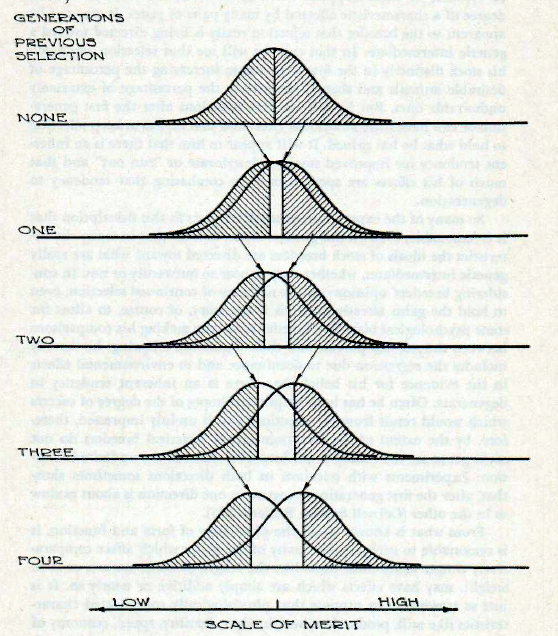
\includegraphics[width=\textwidth]{Figure_19.png}
    \caption{The results expected when selecting simultaneously a low line and a
			 high line for a characteristic only 20 per cent hereditary. Selection is entirelv on the
			 individual's own characteristics except that its parents must have belonged to the
			 same line it did; i.e., there is a pedigree barrier against exchanging animals from one
			 line to the other, no matter what their individual characteristics are. The intensity of
			 selection is such that in each line half are saved to be parents.}
    \label{fig:Lush_Figure_19}
\end{figure}
\index{Environment and heredity|)}
\index{Heritability|)}

\section*{CHANGES IN THE RATE OF IMPROVEMENT BY SELECTION}
\index{Variation!as affected by selection|(}

Whether the rate of progress increases in succeeding generations, or
remains steady, or decreases, depends on changes in the amount of genetic
variance, provided the percentage of culling remains about the
same. The genetic variance changes about as $q(l - q)$ does. It therefore
increases as the frequency of the favorable genes goes from low
values toward .5 and declines as it goes from .5 toward 1.0. The decline
in the rate of progress even then will be very slow, especially if heritability
is not high. It is not often , except when the amount of epistatic
variance is large, that the rate of progress by selection will decline sharply
after only a generation or two. The rate of progress may even increase
sharply after a few generations if the epistatic relations are of a threshold
kind such that at the start most of the population was below some
threshold above which it must rise before the genetic differences could
express themselves freely. Something of this kind seems to have happened
in Payne's selection experiments for bristle number in Drosophila
(Indiana University Studies V, No. 36. 1918) and perhaps in Goodale's
selection for body weight in mice (\textit{Journal of Heredity} 29: 101--12,
1938.)
\index{Variation!as affected by selection|)}

\section*{SELECTION FOR EPISTATIC EFFECTS}
\index{Selection!for epistatic effects|(}

The kinds of gene interaction possible are so numerous that they
defy cataloguing, but the outward results of selecting for them seem to
be typified by what happens when selection favors an intermediate
degree of a characteristic affected by many pairs of genes. It may not be
apparent to the breeder that selection really is being directed toward a
genetic intermediate. In that case he will see that selection improved
his stock distinctly in the first generation, increasing the percentage of
desirable animals and sharply decreasing the percentage of extremely
undesirable ones. But he will see that selections after the first generation
or two have little additional effect and that he has to keep selecting
to hold what he has gained. It will appear to him that there is an inherent
tendency for improved stock to deteriorate or ``run out'' and that
much of his efforts are spent merely in combating that tendency to
degeneration.

So many of the experiences of stock breeders fit this description that
it is reasonable, even on this ground alone, to infer that in many characteristics
the ideals of stock breeders are directed toward what are really
genetic intermediates, whether they appear so outwardly or not. In considering
breeders' opinions on the necessity of continued selection, even
to hold the gains already made, it is necessary, of course, to allow for
some psychological bias. The breeder is usually making his comparisons
between the \textit{selected} parents and their \textit{unselected} offspring; he thereby
includes the regression due to dominance and to environmental effects
in the evidence for his belief that there is an inherent tendency to
degenerate. Often he has built unjustified hopes of the degree of success
which would result from his selections and is unduly impressed, therefore,
by the extent of his disappointments. Practical breeders do not
often get to see the results of deliberate selection in the undesired direction.
Experiments with selection in both directions sometimes show
that, after the first generation, progress in one direction is about as slow
as in the other (Cornell Station Bulletin 533).

From what is known about the physiology of form and function, it
is reasonable to suppose that many of the genes which affect comparatively
simple anatomical traits like the length of bone, stature, or even
weight, may have effects which are simply additive or nearly so. It is
just as reasonable to suppose that physiologically complicated characteristics
like milk production, health, vigor, fertility, speed, economy of
gain, etc., are dependent for their maximum expression on a harmonious
balancing of the magnitudes and functions of many different
organs. If that is so, then it must often happen that in selecting for
maximum production in these economically important characteristics
the breeder really is selecting for balanced or intermediate sizes of
lungs, of heart, of digestive tract, etc. As a purely mechanical illustration,
consider how with an automobile the maximum mileage per gallon
of gasoline is not obtained at the very slowest speeds and certainly
not at the very highest speeds. Moreover the value of the driver's time
or the urgency of the errand may make the most desirable speed something
other than that which is most economical of gasoline. In most
stock judging there is much emphasis on symmetry and ``balance'' in
the animal as a whole. Perhaps this is more justified than would be the
case if each gene were consistently desirable or consistently undesirable,
as is inferred in many discussions of applied genetics.

\index{Selection!for intermediate|(}
A good example of a characteristic which is optimum at an intermediate
value is the thickness of the back fat in hog carcasses to be sold
in the bacon trade. In Sweden since 1938 the optimum thickness of fat
over the middle of the back has been considered to be 29 to 31 mm.\footnote{For
details sec: Activities of the research statiom for testing swine breeding
stock during 1937 (Translated title), Bui. 487 from "Centralanstalten f\"or
f\"ors\"oksv\"asendet p{\aa} Jordbruksomr{\aa}det" Stockholm, 1938.}
When the thickness is already near this optimum, an increase or
decrease of one millimeter changes the carcass value only a little. But
when the fat is already extremely thin, or much too thick, then one
more or one less millimeter in thickness makes a large change in the
value of the carcass. For example, an increase of one millimeter would
change the carcass score as follows when the initial thickness is as
shown:

\begin{table}[h]
	\centering
	\begin{tabular}{cc}
	Initial thickness		& Change in score \\
	13 mm.					& 3.5 points increase \\
	19 mm.					& 2.2 points increase \\
	27 mm.					& .5 points increase \\
	33 mm.					& .6 points decrease \\
	36 mm.					& 1.3 points decrease \\
	44 mm.					& 3.1 points decrease \\
	\end{tabular}
\end{table}

\noindent
Thus a gene which will increase backfat thickness one millimeter
would be highly desirable in a population where the carcasses range
between 14 and 22 millimeters in thickness. Most of its effects in that
population would be additive and selection for the relatives of those
which have the best carcasses would increase the frequency of that gene.
In a population which averages 30 mm. in thickness such a gene would
lower desirability of its possessor in about as many cases as it would
increase desirability. Its average effect would be zero, all of the individual
effects it actually makes would be epistatic, and selection would
not tend consistently either to increase or decrease its frequency. In a
population in which the thickness already ranges from 36 to 44 mm.,
such a gene would be undesirable, nearly all of its effects would be additive,
and selection would tend to lower its frequency.

The emphasis laid on symmetry, balance and proportion in most
animal husbandry judging, the physiological and mechanical relations
between the functioning of an animal and the dimensions of its parts,
the fact that so many chemical reactions in metabolism are of a threshold
nature, and similar considerations, indicate that situations in which
the intermediate is favored over either extreme are rather common,
although there may be some strictly linear relations, too. Probably
there are many situations in which the regression of desirability on
genotype is curvilinear but the curvature is slight enough within the
limits of that population that a straight line comes fairly close to
describing the facts and selection would change gene frequency a long
way before reaching an optimum or some threshold beyond which
further changes in gene frequency would have no effect on average outward
desirability.

\index{Equilibrium between selection and mutation!when selecting for an intermediate|(}
The idea of a desirable intermediate may be extended, and indeed
must be extended, to cover cases where two or more intermediates
widely separated on the genetic scale may each be more desirable than
the genotypes immediately adjacent to them and yet need not be exactly
equal in their own desirability. Desirability for the purposes of the
animal breeder (or ``fitness,'' if the problem is being considered from
the evolutionary point of view) is such a complex thing that there must
be many cases where a certain magnitude of a characteristic fits its possessor
better for a certain purpose than magnitudes just a little larger or
a little smaller would, and yet a magnitude very distinctly larger or
smaller would fit it better for some other purpose or ecological niche.
A crude illustration of that is milk production in cattle. There are
regions, especially in the corn belt, where both specialized beef production
and specialized dairy production can be profitable systems of farming.
The most desirable milk production for a cow used in the
specialized beef farming is just enough to feed her calf well. More than
that would lead to some trouble with spoiled udders, etc. But the peak
of desirability in specialized dairy production is far different. There
may, of course, be other farms where the physical resources and the
aptitudes of the owner make an intermediate milk production most
desirable. In that case there might exist, even in the same region, several
different peaks of desirability in milk production. Another example is
size in horses. In most of the United States there is not much demand
for a horse which is too big to be a children's pony but too small to be a
good saddle horse for a grown person. If it were small enough (like the
Shetlands) or large enough (like the American Saddle Horse), it might
have a high cash value; but, if it is one of the ``in-between'' kinds, there
may be few who will want it. Again, if it were between the ideal for
saddle horses used for pleasure and the ideal for cavalry horses, or if it
were too big for a cavalry horse, it would be at a disadvantage compared
with those which were just the right size. Figure~\ref{fig:Lush_Figure_20} shows such a
situation diagrammatically, so far as it can be pictured for variation
along one dimension.

\begin{figure}
	\centering
    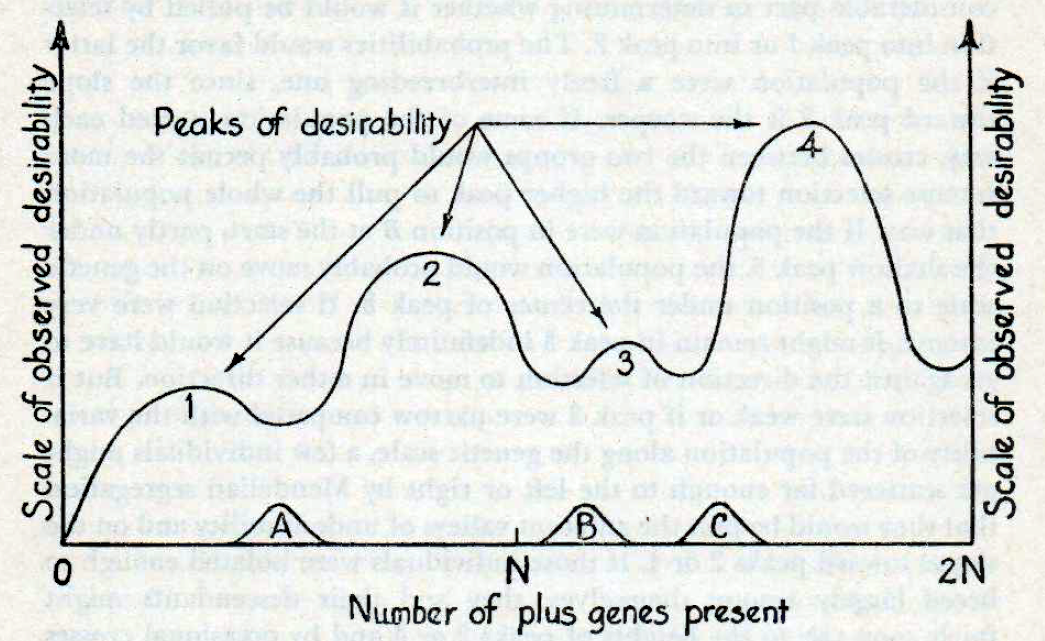
\includegraphics[width=\textwidth]{Figure_20.png}
    \caption{Illustrating the case of several different genetic intermediates (l, 2, 3.
			 and 4), each of which is more desirable than the genotypes which are most nearly like
			 it. \textit{A}, \textit{B}, and \textit{C} are populations whose averages are at 
			 different places along the genetic scale.}
    \label{fig:Lush_Figure_20}
\end{figure}

If the animal's position on the horizontal scale can be seen or measured,
the situation offers no new complications over the general case
already described for selection directed toward an intermediate. But if
only its position on the vertical scale of outward desirability can be
observed\footnote{Thus, in the example about length of leg and speed in race horses, one might
have abundant records on the actual racing speed of many horses but no information
at all about the lengths of their legs. Then one would know in detail whether they
were fast or slow (their outward desirability) but would know nothing about whether
their legs were long or short (their position on the horizontal scale). Two horses
might be equally slow, one because its legs were too short and the other because its
legs were too long, but a man knowing only the record of speed would not know
whether they were alike or far apart on the genetic scale} and the horizontal scale
is long enough for the peaks of desirability to be distinctly separated from each
other by deep valleys, then a new kind of complexity occurs. That is shown by \textit{A}, \textit{B}, and \textit{C},
which represent different positions along the genetic scale in which the
genotypes of a population might happen to be distributed when selection
began. If a population were in position \textit{A}, immediately in the valley
of undesirability between peaks 1 and 2, chance would play a
considerable part in determining whether it would be pulled by selection
into peak 1 or into peak 2. The probabilities would favor the latter
if the population were a freely interbreeding one, since the slope
toward peak 2 is the steeper. If some of the population started each
way, crosses between the two groups would probably permit the more
intense selection toward the higher peak to pull the whole population
that way. If the population were in position \textit{B} at the start, partly under
the shallow peak 3, the population would probably move on the genetic
scale to a position under the center of peak 3. If selection were very
intense, it might remain in peak 3 indefinitely because it would have to
go again st the direction of selection to move in either direction. But if
selection were weak or if peak 3 were narrow compared with the variability
of the population along the genetic scale, a few individuals might
get scattered far enough to the left or right by Mendelian segregation
that they would be past the adjacent valleys of undesirability and on the
slopes toward peaks 2 or 4. If those individuals were isolated enough to
breed largely among themselves, they and their descendants might
fairly soon rise to the heights of peaks 2 or 4 and by occasional crosses
back with the rest of the population might pull the whole population
over to their peak. If, however, the occasional individuals which are
different from their population in enough genes to be past the valleys
interbred freely with the whole population, their offspring would probably
be pulled back into the general population because the mates
would usually be near the population average.
\index{Equilibrium between selection and mutation!when selecting for an intermediate|)}

Whether the population would remain in peak 3 would therefore
depend on the balance between selection, the degree to which the population
tends to separate into rarely interbreeding groups, and the height
and width of peak 3 and the depths of the valleys surrounding it. The
more intense the selection, the more the population would tend to be
held in that peak. The only force tending actively to get it out of that
peak to where it might perhaps find the road to a higher peak is chance
at segregation causing gene frequency to vary in a random direction.
That is a very weak force in large freely interbreeding populations but
may become powerful in a population highly subdivided into small
groups which rarely interbreed. This latter condition leads to some
mild inbreeding which, under some circumstances, may be necessary to
get a population out of a peak where selection has carried it. If the
population were at position \textit{C} when selection began, selection would be
almost certain to carry it to peak 4. There would be no need of inbreeding
to help in that.

This may explain some of the surprising effects sometimes observed
when crossing distinct strains or races. Crossing race \textit{A} and \textit{B} would
give a population with gene frequencies putting it nearly in the center
of peak 2 and would be considered a ``lucky nick .'' On the other hand,
crossing a race already in peak 2 with one already in peak 4 would give
a race with gene frequencies which would put it near the much lower
peak 3. The unfavorable effect might not show in the first generation of
the cross, since each race contributes a full set of its genes, and there is
often enough dominance of the favorable genes to furnish a margin of
safety. But if the first crosses were interbred, the decline in merit from
$F_1$ to $F_2$, when the combinations of genes which worked well together
were scattered, might be extreme. How often this actually happens is
open to question but it points toward a general principle, valid when
epistatic effects are important, that in attempting to perpetuate the
good qualities of an individual it should be mated to members of the
same race or local strain rather than to equally good individuals from
unrelated races where the gene frequencies and combinations may be
widely different. This is the principle of ``linebreeding'' (\textit{\textbf{Chapter 23}}).
Crosses with unrelated or distantly related races may sometimes be
advantageous, too, in originating new lines with desirable combinations
but should always be considered experimental and venturesome, rather
than a dependable general practice.

Desirability for the purposes of the breeder, or fitness in terms of
evolution, depends on many different characteristics, each of which
may have intermediate peaks of desirability. The interdependence of
these on each other's magnitudes increases tremendously the possibilities
for such peaks of desirability where all adjacent genotypes which
might be reached easily by Mendelian segregation in a freely interbreeding
population are less desirable. Figure~\ref{fig:Lush_Figure_20} is a rough sketch of
that, showing variability in only one characteristic. Figure 21 shows the
interplay of variation in two dimensions on desirability, ·which is pictured
as the height of an irregular surface. By observing the increased
complexity of Figure~\ref{fig:Lush_Figure_21} over that of Figure~\ref{fig:Lush_Figure_20}, one can imagine how
complex the situation may be in reality where adaptation or desirability
depends on variation in \textit{n} dimensions and \textit{n} is a large number!

While it appears impossible ever to know enough about the genes
and their physiology and their interplay with environmental circumstances
to know a population's position exactly in all n dimensions of its
adaptability, or to explore the surrounding terrain clearly enough to
know whether there is a higher peak of desirability nearby which might
be reached, yet the general consequences of selection in such a situation
are fairly clear. Selection when first applied will quickly (in terms of
generations) carry the population up the steepest slope of increasing
desirability to the nearest peak in that direction. Selection cannot carry
the population across a deep intervening valley of lessened desirability
to reach a peak of higher desirability on the other side. Only chance
wandering of gene frequency against selection can do that, and this
chance wandering is a very feeble force except when there is considerable
inbreeding. The terrain is apt to be extremely rugged and irregular
in places where two or more genes which individually have very
minor effects may in certain combinations have extremely important
effects on desirability. This gives rise to surprising ``nicking'' effects
which can hardly be seized by selection alone if they are dependent on
more than three or four genes which separately have undesirable effects.

\begin{figure}
	\centering
    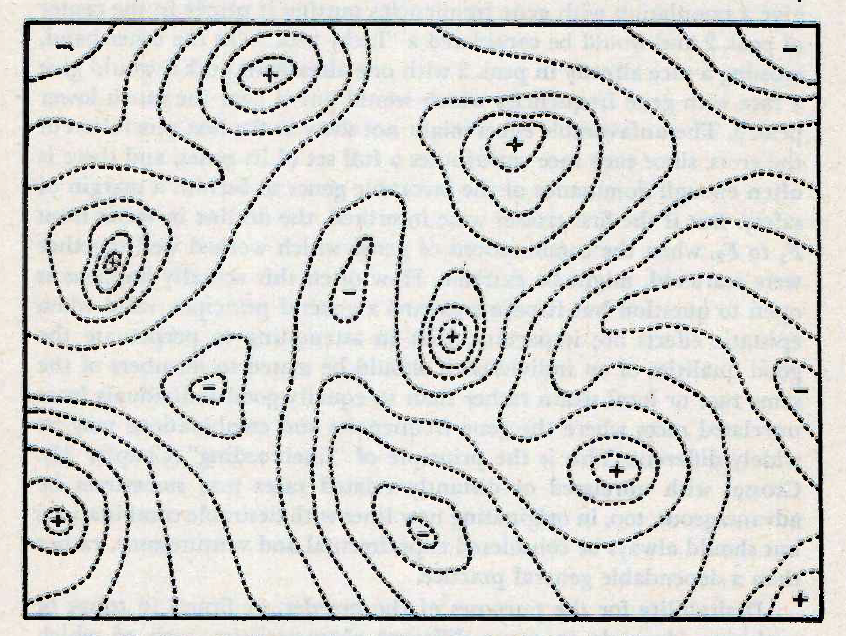
\includegraphics[width=\textwidth]{Figure_21.png}
    \caption{Contour diagram showing how the level of desirability may depend on
			 genetic variability in two different characteristics. Plus signs indicate peaks, and
             minus signs indicate hollows. Selection can carry a population up a slope of c  ontinuously
             increasing desirability but cannot carry it down a slope and across an intervening
             valley to reach a still higher peak (After Wright in \textit{Proc. Sixth Intenat.
             Cong. Genetics}).}
    \label{fig:Lush_Figure_21}
\end{figure}

As a result of the power of selection to carry populations into these
peaks and its inability to get the population out again, most characteristics
which have been under selection for many generations may be
expected already to be in some of those peaks. It is only when selection
in a new direction is just beginning that the position of the population
is as apt to be on a slope ready for rapid progress as it is to be in a peak.
As ideals change with economic or other conditions, peaks will sometimes
change to valleys or the reverse, thus releasing the population
from its peak and permitting rapid progress in some new direction for a
time. To some extent this surface of desirability is always changing, like
that of the sea, so that the peaks do not remain peaks forever. Yet the
rate of such change may perhaps be so slow that, except for changes in
ideals which are caused by changes in economic conditions, it should be
likened more fairly to geological changes in the heights of mountains
and plains.
\index{Epistatic effects|)}
\index{Selection!for epistatic effects|)}
\index{Selection!for intermediate|)}

\section*{SELECTION FOR MANY CHARACTERISTICS AT ONCE}
\index{Scoring|(}
\index{Selection!indexes|(}
\index{Selection!tandem method|(}

The practical animal breeder must consider many different characteristics
in his selections. Some of these are independent of each other
or nearly so; others are positively correlated so that selection for one of
them brings with it a little improvement in the other, although, even if
\textit{x} and \textit{y} are correlated rather closely, selection for \textit{x} indirectly by
selecting for \textit{y} is less effective than selecting for \textit{x} directly if that is possible.
Others are negatively correlated with each other. This makes it a little
harder to select for both of them at once than it would be if they were
independent. Some characteristics are much more important than others.
This needs to be taken into account in balancing excellencies in one
respect against deficiencies in other respects when deciding whether to
keep or cull the animal. The fact that several things must be considered
lowers the intensity of selection possible for each of them, but there is
no escape from that so long as all those things have something to do
with the net desirability of the animal to the breeder or to his
customers.

\index{Culling levels|(}Culling may be done in at least three general ways. The first or tandem
method is to select for one characteristic at a time until that is
improved, then for a second characteristic, later for a third, etc., until
finally each has been improved to the desired level. The second method
is to cull simultaneously but independently for each of the characteristics.
This amounts to establishing for each characteristic culling levels,
below which all individuals are culled, no matter how good are in
other characteristics. The third method is to establish some kind of a
total score or selection index to measure net merit. This would be done
by adding The animal's score for its merit in \textit{x} to its scores for merit in \textit{y},
in \textit{z}, etc. Then those with the poorest total scores would be culled.
Figure~\ref{fig:Lush_Figure_22} illustrates the total score method where two characteristics are
involved.

The tandem method is by far the least efficient of the three, even
when the characteristics are not affected by any of the same genes and it
can be assumed that the improvement made in the first one will not
be lost later while selecting for improvement in the others. Selecting for
one thing at a time will improve that one thing faster than can be done
by any other method of selection, but while that is being done the other
things must wait. Where other things must be improved also, the
improvement made in the first characteristic while it was under selection
must be divided by the whole number of generations necessary to
improve them all in order to get the average rate of improvement in
that one thing. In the simple case in which n characteristics are independent
and equally important, the average improvement per generation
in each will be only one nth of the improvement which is made in
it in the generations when it is the sole object of selection. In this case
the selection index method is $\sqrt{n}$ times as efficient as the tandem
method.

The selection index method is more effective than the method of
independent culling levels because it permits unusually high merit in
one characteristic to make up for slight deficiencies in the other. When
culling by the total score method under the simple conditions of \textit{n} independent
and equally important characteristics, selection for each characteristic
will be $\frac{1}{\sqrt{n}}$ as intense as if all the efforts of selection could
have been concentrated on that characteristic alone.

Under the method of independent culling levels, if \textit{w} is the fraction
of the population which must be saved for breeding, then the intensity
of selection for each characteristic is the same as if selection were directed
at that alone but the fraction which must be saved were $\sqrt[n]{w}$. For
example, if length of body and soundness of feet and legs are uncorrelated
in swine, and a breeder must save 10 per cent of his gilts for breeding
purposes, he can save the 10 per cent with the very longest bodies if
he selects for that alone, or the 10 per cent with the soundest feet and
legs if he selects for that alone, but only 1 per cent of his gilts will be in
the best 10 per cent in both respects. If he pays equal attention to both
things, he must save all gilts which are in the 32 per cent which are
longest and are also in the 32 per cent with best feet and legs if he is to
save IO per cent of his gilts altogether. If he takes quality also into
account, and if quality is not correlated with body length or with
excellence of feet and legs, he will have to save from among the best 46 per
cent (instead of 32 per cent) in each trait in order to have IO per cent of
the best in all three respects. Four traits would increase this to 56 per
cent instead of 46 per cent. If the traits are positively correlated with
each other, the intensity of selection for single traits will not fall off
quite so fast with increasing \textit{n} as these formulas indicate; but, if the
traits are negatively correlated, the intensity of selection for each will
fall off a little faster.

\begin{figure}
	\centering
    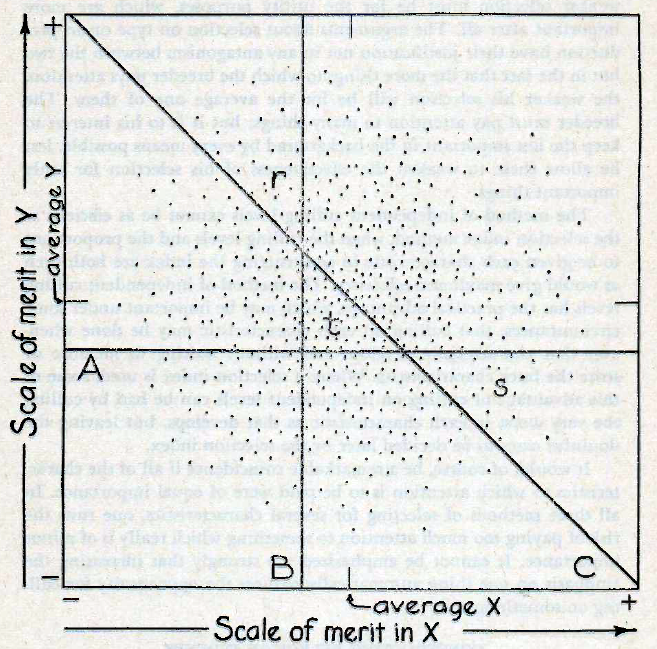
\includegraphics[width=\textwidth]{Figure_22.png}
    \caption{Superiority of culling on total score as compared with culling independently
			 first for one characteristic and then for another. Each dot represents an individual.
			 Merit in \textit{x} is not correlated with merit in \textit{y}. \textit{A} represents the level of merit
			 in characteristic \textit{y} below which all individuals are culled when \textit{y} is considered
			 independently. Similarly, \textit{B} represents the independent culling level for merit in \textit{x},
			 all individuals to the left of \textit{B} being culled. \textit{C} represents a level of culling on total
			 score, with \textit{x} and \textit{y} being regarded as equally important, which would result in keeping
			 an equal fraction of the population. Animals in areas \textit{r} and \textit{s} would be kept when
			 culling on total score but would be discarded when culling independently on \textit{x} and
			 \textit{y}, while the reverse would be true of the animals in area \textit{t}. The fate of the animals
			 in the other four areas would not be altered by changing the method of culling. If \textit{x}
			 and \textit{y} were not equally important the example is still valid, but the slope of line \textit{C}
			 would be different (Brier \textit{et al.}, pages 153--60, in \textit{Proc. Amer. Soc. An. Prod.} for 1940}
    \label{fig:Lush_Figure_22}
    \index{Selection!tandem method|)}
\end{figure}

Here lies the real damage done by paying attention to \index{``Fancy points''}``fancy
points'' in selection; namely, that the more attention given to them, the
weaker selection must be for the utility purposes, which are more
important after all. The arguments about selection on type or on production
have their justification not in any antagonism between the two
but in the fact that the more things to which the breeder pays attention,
the weaker his selection will be for the average one of them. The
breeder must pay attention to many things; but it is to his interest to
keep the less important in the background by every means possible, lest
he allow these to weaken the effectiveness of his selection for truly
important things.

The method of independent culling levels cannot be as efficient as
the selection index method, when the culling levels and the proportions
to be given each characteristic in constructing the index are both such
as would give maximum efficiency. The method of independent culling
levels has the practical advantage, which may be important under some
circumstances, that culling on each characteristic may be done whenever
that characteristic develops and without waiting to measure or
score the later characteristics. Where a selection index is used, some of
this advantage of culling on independent levels can be had by culling
the very worst in each characteristic as that develops, but leaving the
doubtful cases to be decided later by the selection index.

It would, of course, be a remarkable coincidence if all of the characteristics
to which attention is to be paid were of equal importance. In
all three methods of selecting for several characteristics, one runs the
risk of paying too much attention to something which really is of minor
importance. It cannot be emphasized too strongly that increasing the
emphasis on one thing automatically reduces the opportunity for culling
on something else.
\index{Culling levels|)}
\index{Scoring|)}

\section*{CONSTRUCTING SELECTION INDEXES}
\index{Heritability|(}
\index{Heritability!methods of estimating}

The principles of constructing selection indexes designed to make
maximum improvement, are those of multiple regression where it is
desired to predict as accurately as possible an unknown or ``dependent''
variable from two or more known (independent) variables. In this case
the dependent variable is the animal's net genetic merit or breeding
value, while its various characteristics or even the characteristics of its
relatives are the independent variables.

Four bits of information are needed for each characteristic. 1. The
average amount which a given variation in that characteristic actually
raises or lowers the net phenotypic merit of the animal. This we may
call the \textit{importance} of the characteristic. 2. The \textit{heritability} of each
characteristic is important because it is the average fraction of phenotypic
improvement we get in the offspring for each unit of phenotypic
merit in the selected parent. 3. \textit{Genetic correlations} between that 
characteristic and the others may arise if some of the same genes affect two
or more of them. These will mean that selection for characteristic \textit{x} will
help or hinder improvement in characteristic \textit{y}, as compared with what
would happen if they were independent. 4. \textit{Phenotypic correlations}
between that characteristic and the others will exist if some of the same
environmental incidents have affected them. This, in combination with
differences in heritability, may even lead to some characteristics being
useful mainly as indicators of the kind of environment under which
more important characteristics developed.

A quantitative example of the idea of relative importance is the
finding by Winters (\textit{The Empire Jour. of Exp. Agr.} 8:259--68, 1940)
that one pound of wool is worth 3.4 pounds of lamb. The relative
importance of each characteristic may need to be established separately
for each kind of animal, each region, each type of farming, and almost
for each breeder. Naturally this job is never done permanently but
needs to be reviewed whenever the market demands and premiums
make any large and presumably permanent change. Discussions about
what is ``the right type'' to breed mainly concern the relative importance
of different characteristics, although they have in them something
of the other three bits of information also.

Heritability can be approximated by doubling the intrasire regression
of offspring on their dams. This requires data on several hundred
pairs and is not likely to be within the reach of the individual breeder,
but from his general observations he can get a rough idea of the relative
heritability of two characteristics by observing whether the offspring
generally tend to resemble their parents rather closely or slightly
in each of these.
\index{Heritability|)}

The genetic correlation between two characteristics on the same animal
can be measured by observing a large number of pairs of closely
related animals and correlating characteristic \textit{x} in one member of the
pair with characteristic \textit{y} in the other. This requires large numbers, and
the estimates have high sampling errors. It is the bit of information
most likely to be lacking when an index is to be constructed.

The environmental correlation between two characteristics can be
had by correlating the two characteristics on the same animal and subtracting
their genetic correlation obtained as above.

Occasionally it is profitable to pay more attention to a highly
hereditary characteristic which is of limited economic importance than
to a slightly hereditary one, the variations in which affect the value of
the individual animal more strongly. This is because heritability is the
fraction which one gets of what he reaches for when selecting the parents,
and importance measures the value of that for which he is reaching.
One will have more net profit by getting 50 per cent of something
which is worth 20 cents than by getting 30 per cent of something which
is worth 25 cents! It is a question of deploying the available efforts and
resources so as to secure maximum returns.

Because of this relation between heritability and importance, the
different characteristics in a selection index should be given emphasis
in proportion to their heritability times their importance, rather than
in proportion to either one alone. This will be completely true if the
characteristics are not correlated. If the characteristics have strong
environmental and genetic correlations among themselves, this might
alter the size and could even reverse the signs of the attention to be paid
to each characteristic when constructing a selection index. This is just a
special case of the well-known fact that in a multiple regression equation,
strong correlations among the independent variables can alter
greatly the net regression coefficients from what they would be if all the
independent variables were uncorrelated with each other. Emphasizing
each characteristic in proportion to the product of its heritability and
its importance is as good an approximation to the proper weights as is
possible in most cases.

The few studies yet made seem to indicate that if heritability and
importance are known with rough accuracy, the efficiency of the index
based on them will not be changed much by the intercorrelations
between the variables, although the relative importance and even the
sign of some of the weights may be changed much. As an example in a
swine breeding experiment at the Iowa Agricultural Experiment Station,
a selection index was first constructed using only the importance
of the items and the observed phenotypic correlation between litter
mates. It was: $I = 1/3W + S + P + .303\bar{W} + 1.667\bar{S}$ where
$W$ is weight at 180 days, $S$ is score for market desirability, $P$
is productivity of dam, $\bar{W}$ is average weight and $\bar{S}$ is
an average score of the litter in which the pig was born. L. N. Hazel's
analysis\footnote{\textit{Genetics} 28:476--490. 1945} of the data which
were then collected in the next few years of the experiment indicated
that the most efficient index would have been:

\[I^\prime = .3W - .5S + .5P + .270\bar{W} + .605\bar{S}\]

The coefficients in the two indexes are markedly different, especially in
the reversed sign for the coefficient of $S$, yet the efficiency of $I$ was .364
and that of $I^\prime$ was .404, which is larger, but not greatly so. By efficiency
is meant that progress by selecting exactly according to $I$ would make
progress .364 as fast as could be made by the same percentage of culling
if the genotype of every pig were known exactly.
\index{Selection!indexes|)}

\section*{SUMMARY OF RESULTS EXPECTED FROM MASS SELECTION FOR NET MERIT}

Mass selection is expected to cause the average of each generation
to exceed the average of the preceding generation by an amount ($M$)
which is equal to the heritability fraction $\frac{\sigma_G^2}{\sigma_O^2}$
of the selection differential ($S$), the latter being the average
merit of those selected to be parents minus the average of the whole generation
from which they were taken.

There is also a little deterioration from mutation, but this is too
small to be considered further in problems of animal or plant breeding,
although it may be important in evolutionary considerations.

When selection is first begun there will also be some temporary gain
from epistatic effects. This will be something less than half of
$S \times \frac{\sigma_I^2}{\sigma_G^2 + \sigma_D^2 + \sigma_I^2 + \sigma_E^2}$.
It will tend to disappear with each generation of segregation and recombination
and thus, unless constantly renewed by fresh selection, tends to disappear soon
after selection is relaxed.

The obstacles to rapid progress naturally fall into two groups: (1)
Circumstances or practices which make $S$ small and (2) circumstances
or practices which make $\sigma_G^2$ small or $\sigma_D^2$, $\sigma_I^2$, or
$\sigma_E^2$ large, thereby lowering heritability. Although \textit{M} may
perhaps be small, it will not be zero, provided both $S$ and $\sigma_G^2$
have positive values.

Among things which may make $S$ small are:
\begin{enumerate}[topsep=0pt, partopsep=0pt]
\item Perhaps only a small fraction can be culled. Remedies: Anything
which will improve the health of the herd and reduce deaths from
disease or accident; earlier breeding and quicker rebreeding of females,
and anything else which will increase the number of offspring raised
annually per 100 females.

\item The population may be so uniform that the difference between
those selected and those rejected cannot be large. Remedy: Sometimes
one can change the environment so that genetic differences may express
themselves more fully and be magnified. Outcrossing may help.

\item The breeder may be careless about his cullings or changeable in
his ideals. This makes the selection more like discarding at random or
at least more like the top than the bottom of Figure~\ref{fig:Lush_Figure_17}.
Remedy: More care in deciding on the ideals, more attention to detail, planning the
cullings and selections well in advance of the time when they must
actually be made.

\item The measures or yardsticks of individual merit may not be definite
or simple. This has the same effect as 3. Remedy: Clearer and more
quantitative definition of goals, more systematic scoring, grading or
classifying at regular ages or dates, simple but systematic records of
production where possible.

\item The breeder may be trying to pay attention to too many things
in his selections, thus weakening the intensity of selection for the more
important things. Remedy: Resolutely keeping minor things in the
background, perhaps using a selection index.

\noindent
Among things which make heritability low are:

\item $\sigma_G^2$ may be small. Remedies: An outcross to a relatively unrelated
stock having some desirable characteristics which are absent or
rare in the breeder's own herd may restore genetic variability. Probably
most breeds of farm animals still have enough genetic variability
within them that crossing with other breeds is not necessary for making
a large amount of further improvement. Introducing blood from outside
the breed cannot be done in most breeds under the prevailing
standards of purebreeding, although outcrossing within the breed is
always possible. Inbreeding a population without discarding any of the
lines tends toward doubling $\sigma_G^2$ but puts most of it between lines and
tends to extinguish genetic variance within lines. When the better lines
are selected and the poorer lines are discarded, the genetic variance
then remaining is likely to be smaller than was in the population when
the inbreeding began. Sometimes it may be possible to alter the environment
enough to magnify the outward differences between genetically
different individuals, particularly where thresholds are involved, but it
may be difficult to find the environmental changes which will do that.

\item $\sigma_E^2$ is usually large except for a few characteristics such as colors
and things which are fairly simple anatomically, such as the dimensions
of the bones, shape of head, set of ear, etc. Remedy: Keep the environment
alike for all individuals as far as is economical, correct for the
effects of the more important differences in environment which did
occur, use lifetime averages where those are practicable, and give some
attention to the merits of relatives and progeny.

\item $\sigma_D^2$ may be large. This can be an important obstacle only where
most of the undesired genes are recessives already rare, and in pairs of
genes where the heterozygote is preferred over both homozygotes. Remedy:
Consider the relatives. The collateral ones usually give more help
in this respect than the ancestors do. The progeny are still more
informative, especially if they are inbred.

\item $\sigma_I^2$ may be large. This seems likely to be important only where
the population has already been under selection for many generations.
Remedy: Consider the relatives and progeny. Inbreed enough to form
distinct families, only rarely making crosses between them. Breed within
the family as long as its average merit is good.
\end{enumerate}

These ways of overcoming partially the obstacles to progress by
mass selection will be considered separately in the following chapters.
The purpose of this chapter has been to describe and explain the results
of unaided mass selection. It alters the population mean almost in proportion
to \textit{n} times the amount it changes gene frequency, n being the
number of genes affecting the characteristic.

The rate of improvement per generation may increase or decrease
in later generations but is not likely to change rapidly unless there is a
considerable amount of epistatic interaction.

Only rarely is mass selection completely ineffective, as when selection
is for a heterozygote, when selection has already carried the population
into a stable epistatic peak, or when selection is within an
entirely homozygous line. Often, however, the rate of progress by mass
selection is slow and could be made more rapid by a judicious use of
relatives and progeny or by more careful control or consideration of the
environment.

\section*{REFERENCES}

The classical cases of selection experiments with higher animals are
those of Castle on the hooded pattern in rats, mostly published from
about 1914 to 1920, and Pearl's experiments on selection for high egg
production in the poultry flock at the Maine Station a little earlier. In
plants the Illinois Experiment Station selections for high and low oil
content and for high and low protein content in corn kernels and
Johannsen's selections in Denmark for seed size in beans are famous
among experiments on selection. For brief accounts of these and other
actual experimental studies of selection, see:

\begin{hangparas}{0.5in}{1}%
Babcock. E. B., and Clausen, R. E. 1927. Genetics in relation to agriculture. pp.
221--31 and 538--50.

Castle, W. E. 1930. Genetics and eugenics. pp. 236--45.

Goodale, H. D. 1938. A study of the inheritance of body weight in the albino
mouse by selection. Jour. Heredity 29:101--12.

Sinnott, E. W., and Dunn. L. C. 1925. Prin. of genetics. pp. 339--46.

Winter, F. L. 1929. Mean and variability as affected by continuous selection for
composition in corn. Jour. Agr. Res. 39:451--76.
\end{hangparas}
\index{Selection|)}